\sloppy
\documentclass[14pt,a4paper,oneside]{extarticle}	% Размер основного шрифта и формата листа
\usepackage{xltxtra}						% Используется для вывода логотипа XeLaTeX
\usepackage{xunicode}						% Кодировка документа
\usepackage{polyglossia}					% Загружает пакет многоязыковой верстки
\newfontfamily\russianfont{Book Antiqua}
%\setmainfont{Liberation Serif}						% Основной шрифт текста
\setmainfont{Book Antiqua}
\setdefaultlanguage{russian}				% Основной язык текста
\setotherlanguage{english}					% Дополнительный язык текста
\linespread{1}							% Межстрочный интервал выбран полуторным
\usepackage[left=2.5cm,
right=1.5cm,vmargin=2.5cm]{geometry} % Отступы по краям листа
\bibliographystyle{ugost2008}

\usepackage{xcolor}
\usepackage{hyperref}
% Цвета для гиперссылок
\definecolor{linkcolor}{HTML}{359B08} % цвет ссылок
\definecolor{urlcolor}{HTML}{799B03} % цвет гиперссылок
\hypersetup{pdfstartview=FitH,  linkcolor=linkcolor,urlcolor=urlcolor, colorlinks=true}

%---------------------------%
%---- Пакеты расширений ----%
%---------------------------%
\usepackage{xcolor}
\usepackage{hyperref}
% Цвета для гиперссылок
\definecolor{linkcolor}{HTML}{359B08} % цвет ссылок
\definecolor{urlcolor}{HTML}{799B03} % цвет гиперссылок
\hypersetup{pdfstartview=FitH,  linkcolor=linkcolor,urlcolor=urlcolor, colorlinks=true}


\usepackage{verbatim,indentfirst}
\usepackage{cite,enumerate,float}
\usepackage{amsmath,amssymb,amsthm,amsfonts}

%---------------------------%
%--- Вставка иллюстраций ---%
%---------------------------%
\usepackage{graphicx}
\usepackage{subfigure}
\usepackage{fontspec}
%\graphicspath{{Images/}}

\begin{document}
%	\pagestyle{empty} %  выключаенм нумерацию
%\setcounter{page}{3}% Нумерация начинается с третьей страницы
%\renewcommand{\contentsname}{\center{Содержание}}
%\tableofcontents

\begin{center}
	%\addcontentsline{toc}{section}{Опыт 8. Движение тела по «мертвой петле»}
	\subsection*{Движение тела по «мертвой петле»}
\end{center}

\begin{figure}[H] 
	\centering 		
	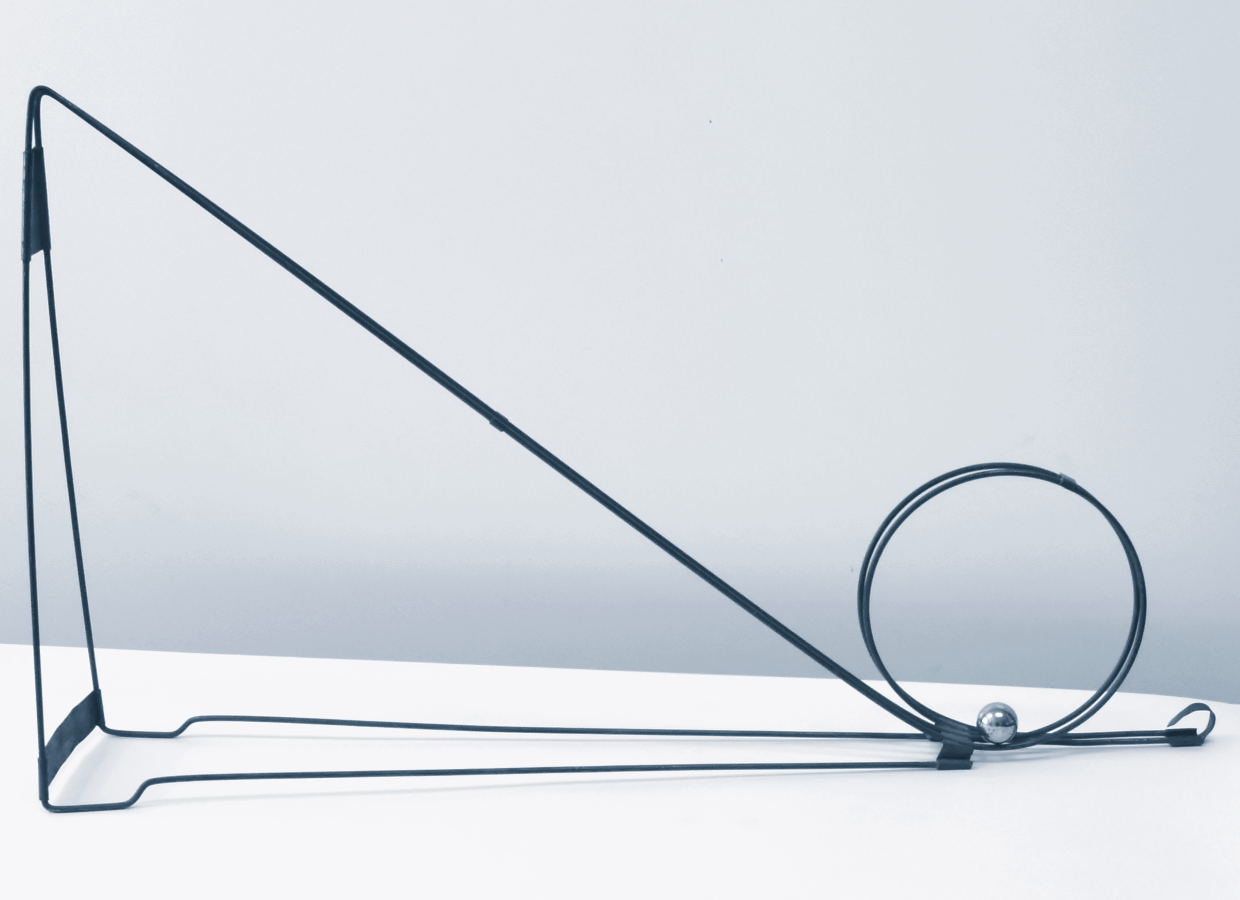
\includegraphics[width=0.75\linewidth]{loop-1.png}
	\caption{Демонстрация взаимосвязи кинетической и потенциальной энергии}
	\label{loop-1}
\end{figure}

\subsection*{\underline{Оборудование:}}

\begin{enumerate}
	\item Лабораторная модель «мертвой петли» (радиус кривизны 8 см).
	\item Стальной шарик диаметром 2 см.
\end{enumerate}

\newpage
\subsection*{\underline{Основные определения:}}

Нестерова петля («мертвая петля») — фигура высшего пилотажа, 
представляющая собой замкнутую кривую в вертикальной плоскости. 
Названа по имени П. Н. Нестерова, впервые в мире выполнившего ее 27~августа~1913~г.

Для того, чтобы материальная точка совершала движение по окружности с центростремительным ускорением $a = v^2/r$, необходимо, чтобы на тело действовала внешняя сила. В представленной демонстрации роль внешней силы играет сила реакции опоры. В соответствии с 3 законом Ньютона на направляющие, вдоль которых движется тело, действует равная по модулю сила давления (сила веса).

В устаревшей литературе можно встретить такие определения: сила, с которой движущаяся материальная точка действует на опору (вес) - это центробежная сила, а сила, с которой опора давит на точку - это центростремительная сила (реакции опоры).
Центробежная сила и центростремительная сила численно равны друг другу и направлены вдоль одной прямой в противоположные стороны, но приложены к разным телам — как силы действия и противодействия.
Определенные таким образом силы, считаются устаревшими понятиями и в современной литературе не используются.
Согласно современным представлениям центробежная сила инерции действует в неинерциальной системе отсчета на движущееся тело, а термин "центростремительная сила" не используется вовсе.

Кинетическая энергия — энергия механической системы, зависящая от скоростей движения ее точек.
Кинетическая энергия $ E_{\text{к}} $ материальной точки измеряется половиной произведения массы $ m $ этой точки на квадрат ее скорости $ v $, т. е. $$ E_{\text{к}}  = \frac{mv^2}{2}. $$ 
Кинетическая энергия механической системы равна арифметической сумме кинетических энергий всех ее точек: 
$$ E_{\text{к}}  = 1/2 \sum  m_i v_i^2.$$ 

Изменение кинетической энергии системы при ее перемещении из положения 1 в положение 2 
происходит под действием приложенных к системе внешних и внутренних сил и равно сумме работ $ A_{\text{внеш}}$ и $ A_{\text{внутр}}$ этих сил на данном перемещении:
$$
E_{\text{к}_{2}} - E_{\text{к}_{1}} = A_{\text{внеш}} + A_{\text{внутр}}
$$
 
Это равенство выражает теорему об изменении кинетической энергии, с помощью которой решаются многие задачи динамики.

\newpage
\subsection*{\underline{Краткое описание:}}

Прибор «мертвая петля» позволяет демонстрировать ряд опытов по динамике движения материальной точки по окружности.
Эти опыты дают возможность выяснить соотношение сил (силы тяжести и реакции рельсов), действующих на катящийся по рельсам шарик и определить, при каких условиях шарик без отрыва преодолеет метрвую петлю.

На приборе сначала демонстрируется три основных опыта: 1) с наивысшей точки $ 1 $ (рис.\ref{loop-2}) наклонных рельсов, когда шарик устойчиво описывает петлю и с некоторой скоростью вылетает с другого конца желоба; 2) с наименьшей высоты $ 2 $ (рис.\ref{loop-2}) наклонной плоскости, когда шарик только описывает петлю, не срываясь с верхней токи, и 3) с еще меньшей высоты $ 3 $ (рис.\ref{loop-2}), когда шарик, не доходя до вершины петли, отрывается от направляющих и движется внутри петли по параболической траектории.

\newpage
\subsection*{\underline{Теория:}}

Рассмотрим этот опыт, не учитывая диссипативные силы (трение шарика о направляющие), и найдем начальное положение (высота $ h $), достаточное для того, чтобы тело преодолело «мертвую петлю».  

\begin{figure}[H] 
	\centering 	
	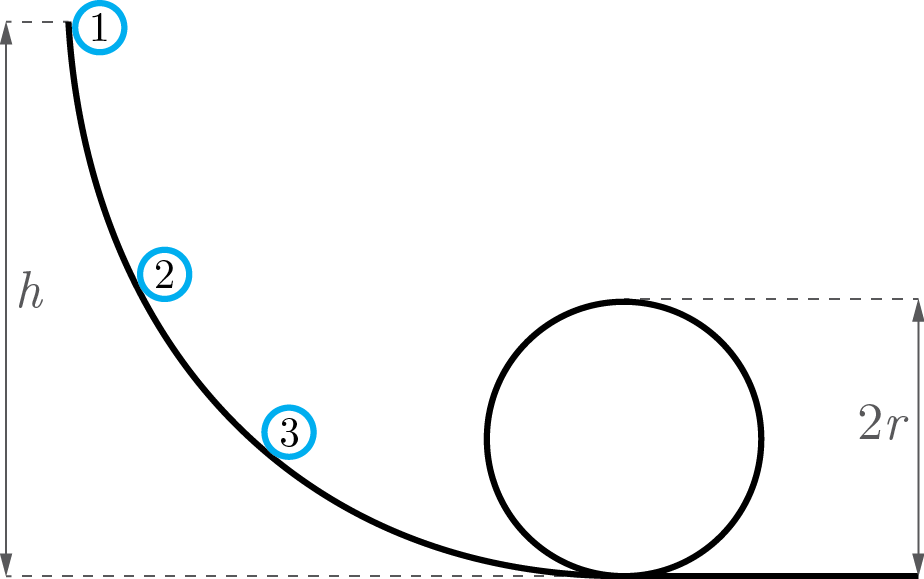
\includegraphics[width=0.5\linewidth]{loop-2.png}
	\caption{Схематичное изображение направляющих, по которым движется точка. Начальные положения тела отмечены точками 1, 2 и 3}
	\label{loop-2}
\end{figure}

Шар в начальный момент времени обладает только потенциальной энергией:
  
\begin{equation}\label{loop-eq1}
E_{\text{п}} = mgh,
\end{equation}
 где $ m $ — масса шарика, а $ h $ — начальная высота спуска.
 
Рассмотрим момент, когда шарик оказывается в верхней точке петли. Будем считать, что скорость тела минимально возможная, тогда сила реакции опоры обращается в ноль.
В этот момент тело обладает центростремительным ускорением, равным ускорению свободного падения $ a_{z} = g $, поскольку именно сила тяжести сообщает телу центростремительное ускорение.
Учитывая эту связь имеем:  
\begin{equation}\label{loop-eq5}
a_{z} = \frac{v^{2}_{2}}{r} = g,
\end{equation}
где $ v_2 $ — скорость шара в верхней точке петли.

Закон сохранения энергии примет вид:
\begin{equation}\label{loop-eq6}
E_{\text{к}_{2}} + E_{\text{п}_{2}} = E_{\text{п}},
\end{equation}
можно записать в следующем виде:
\begin{equation}\label{loop-eq7}
\frac{mv_{2}^{2}}{2} + 2mgr = mgh.
\end{equation}

Необходимо сделать важное замечание о том, что при скатывании шара конечных размеров (нематериальная точка) нужно учитывать его момент инерции $I = 2mR^2/5$, где \textit{R} — радиус шара.
В этом случае в законе сохранения энергии следует добавить слагаемое $$E_\text{в} = I\omega^{2}/2,$$
и тем самым учесть кинетическую энергию вращательного движения тела при скатывании вдоль направляющих.
Однако дальнейшие выкладки приводятся в приближении материальной точки.

Из уравнения (\ref{loop-eq7}) после несложных преобразований получим:
\begin{equation}\label{loop-eq8}
v_{2}^{2} + 4gr = 2gh.
\end{equation}

Если из выражения (\ref{loop-eq5}) выразить $ v_{2}^{2} $ и подставить это соотношение в уравнение (\ref{loop-eq8}), то получим:
\begin{equation}\label{loop-eq9}
h = \frac{5gr}{2g} = 2.5r.
\end{equation}

Таким образом, если высота $ h > 2.5r $, то тело способно преодолеть петлю, однако при условии $ h < 2.5r $ скорости тела окажется недостаточно для полного оборота.

В реальности же равенство $ h = 2.5r $ не выполняется, так как в системе неизбежно появление сил сопротивления.
Из-за трения шарика о металлические рельсы условие прохождения петли примет вид $ h \geq 2.5r $.

\end{document}